\documentclass[mathserif,xcolor=dvipsnames,hyperref={bookmarks=true}]{beamer}
%\documentclass[mathserif,xcolor=dvipsnames,handout]{beamer}
%\usepackage{listings}
\usepackage[scaled]{helvet}
\usepackage{eulervm}
\usepackage{listings}
\usepackage{courier}
%\usepackage{xmpincl}  % http://www.ctan.org/tex-archive/macros/latex/contrib/xmpincl/
%\usepackage{listings}
%\includexmp{byncsa}
\usepackage[binary,amssymb]{SIunits}
\usefonttheme{structurebold}
\usecolortheme[named=Maroon]{structure}
\usetheme{Antibes}
\usecolortheme{lily}
\useoutertheme{infolines}
\setbeamertemplate{navigation symbols}{}
\usepackage{xmpmulti} % for \multiinclude

\newcommand{\mytitle}{Making Creative Commons More Useful by Applying Usage Management}
\newcommand{\myshorttitle}{CC More Useful with Usage Managment}
\newcommand{\myauthor}{Matthew Paul Bohnsack}
\newcommand{\myshortauthor}{Matthew Bohnsack}

% We should look for graphics in these directories
\graphicspath{
{../resources/usecases/usecase1/}
{../resources/usecases/usecase2/}
{../resources/component-design/}
}

% Check this for automating the creation of different files: slides, handouts, etc...
% http://www.pletscher.org/writings/latex/Makefile
% http://www.pletscher.org/writings/latex/beamer.php

% Do this if handouts...
%\usepackage{pgfpages}
%\pgfpagesuselayout{2 on 1}[letterpapper,border shrink=5mm]
%\mode<handout>{\setbeamercolor{background canvas}{bg=black!5}}

\usepackage{default}

\title[\myshorttitle]{\mytitle}
%\subtitle{Including a Usage Management Example in Ruby}
\author[\myshortauthor]{\myauthor}
\institute[UNM]{University of New Mexico\\Albuquerque, New Mexico USA\\[2ex]\texttt{bohnsack@gmail.com}}
%\date{Friday March 25, 2011}

\newcommand{\putat}[3]{\begin{picture}(0,0)(0,0)\put(#1,#2){#3}\end{picture}}

%\lstset{language=bash,rulesepcolor=\color{Gray},frame=shadowbox,basicstyle=\tiny\ttfamily}

\begin{document}

%%%%%%%%%%%%%%%%%%%%%%%%%%%%%%%%%%%%%%%%%%%%%%%%%%%%%%%%%%%%%%%%%%%%%
% Title
%%%%%%%%%%%%%%%%%%%%%%%%%%%%%%%%%%%%%%%%%%%%%%%%%%%%%%%%%%%%%%%%%%%%%
\begin{frame}
    \titlepage
    \begin{center}
        \includegraphics[width=0.24\textwidth]{resources/logos/UNM/UNM_logo_PMS200C.pdf}
    \end{center}
\end{frame}

%%%%%%%%%%%%%%%%%%%%%%%%%%%%%%%%%%%%%%%%%%%%%%%%%%%%%%%%%%%%%%%%%%%%%
\section{Introduction}
%%%%%%%%%%%%%%%%%%%%%%%%%%%%%%%%%%%%%%%%%%%%%%%%%%%%%%%%%%%%%%%%%%%%%
\begin{frame}[t]
    \tableofcontents[currentsection,hideallsubsections]
\end{frame}

    \subsection{Abstract}
    %%%%%%%%%%%%%%%%%%%%%%%%%%%%%%%%%%%%%%%%%%%%%%%%%%%%%%%%%%%%%%%%%%%%%
    \begin{frame}[t]
        \frametitle{Abstract}
    \end{frame}

    \subsection{Motiviation}
    %%%%%%%%%%%%%%%%%%%%%%%%%%%%%%%%%%%%%%%%%%%%%%%%%%%%%%%%%%%%%%%%%%%%%
    \begin{frame}[t]
        \frametitle{Motiviation}
    \end{frame}

    \subsection{Creative Commons}
    %%%%%%%%%%%%%%%%%%%%%%%%%%%%%%%%%%%%%%%%%%%%%%%%%%%%%%%%%%%%%%%%%%%%%
    \begin{frame}[t]
        \frametitle{Creative Commons}
    \end{frame}

    \subsection{XMP}
    %%%%%%%%%%%%%%%%%%%%%%%%%%%%%%%%%%%%%%%%%%%%%%%%%%%%%%%%%%%%%%%%%%%%%
    \begin{frame}[t]
        \frametitle{XMP}
    \end{frame}

    \subsection{Flickr}
    %%%%%%%%%%%%%%%%%%%%%%%%%%%%%%%%%%%%%%%%%%%%%%%%%%%%%%%%%%%%%%%%%%%%%
    \begin{frame}[t]
        \frametitle{Flickr}
    \end{frame}

    \subsection{Usage Management}
    %%%%%%%%%%%%%%%%%%%%%%%%%%%%%%%%%%%%%%%%%%%%%%%%%%%%%%%%%%%%%%%%%%%%%
    \begin{frame}[t]
        \frametitle{Usage Management}
    \end{frame}

%%%%%%%%%%%%%%%%%%%%%%%%%%%%%%%%%%%%%%%%%%%%%%%%%%%%%%%%%%%%%%%%%%%%%
\section{System Design}
%%%%%%%%%%%%%%%%%%%%%%%%%%%%%%%%%%%%%%%%%%%%%%%%%%%%%%%%%%%%%%%%%%%%%
\begin{frame}[t]
    \tableofcontents[currentsection,hideallsubsections]
\end{frame}

    \subsection{Use Cases}
    %%%%%%%%%%%%%%%%%%%%%%%%%%%%%%%%%%%%%%%%%%%%%%%%%%%%%%%%%%%%%%%%%%%%%

    % Use Case #1 %%%%%%%%%%%%%%%%%%%%%%%%%
    \begin{frame}[t]
        \frametitle{Use Case \#1}
        \begin{center}
            % The "[<+>]" thing means totally replace the prior graphic each
            % time.  Otherwise the default behavior is to stack all graphics
            % on top of each other.
            \multiinclude[<+>][format=pdf,graphics={width=0.51\textwidth}]{usecase1}
        \end{center}
    \end{frame}

    % Use Case #2 %%%%%%%%%%%%%%%%%%%%%%%%%
    \begin{frame}[t]
        \frametitle{Use Case \#2}
        \begin{center}
            \multiinclude[<+>][format=pdf,graphics={width=0.9\textheight}]{usecase2}
        \end{center}
    \end{frame}

    \subsection{Component Design}
    %%%%%%%%%%%%%%%%%%%%%%%%%%%%%%%%%%%%%%%%%%%%%%%%%%%%%%%%%%%%%%%%%%%%%

    % Compliance Checking Tool %%%%%%%%%%%%
    \begin{frame}[t]
        \frametitle{Compliance Checking Tool}
        \begin{center}
            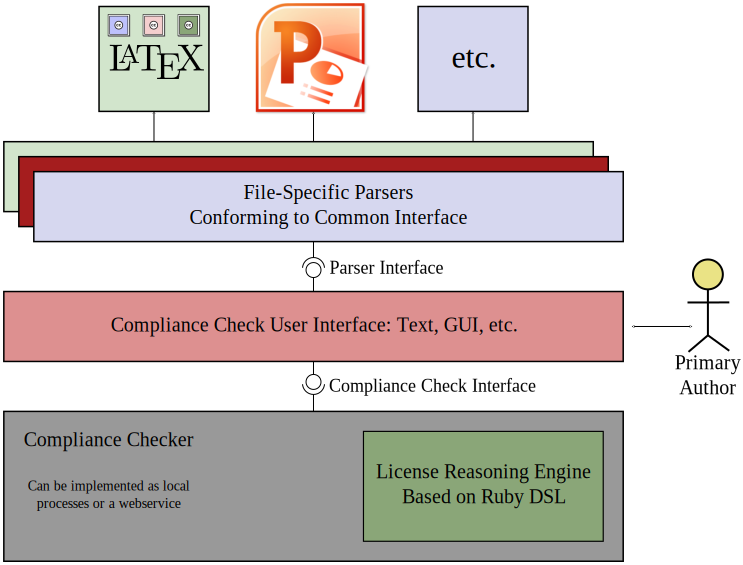
\includegraphics[width=0.9\textheight]{compliance-checking-tool.pdf}
        \end{center}
    \end{frame}

    % License Reasoning Engine %%%%%%%%%%%%
    \begin{frame}[t]
        \frametitle{License Reasoning Engine}
    \end{frame}

    % CC+ Broker Service %%%%%%%%%%%%%%%%%%
    \begin{frame}[t]
        \frametitle{CC+ Broker Service}
    \end{frame}

%%%%%%%%%%%%%%%%%%%%%%%%%%%%%%%%%%%%%%%%%%%%%%%%%%%%%%%%%%%%%%%%%%%%%
\section{Implementation}
%%%%%%%%%%%%%%%%%%%%%%%%%%%%%%%%%%%%%%%%%%%%%%%%%%%%%%%%%%%%%%%%%%%%%
\begin{frame}[t]
    \tableofcontents[currentsection,hideallsubsections]
\end{frame}

%%%%%%%%%%%%%%%%%%%%%%%%%%%%%%%%%%%%%%%%%%%%%%%%%%%%%%%%%%%%%%%%%%%%%
\section{Future Work}
%%%%%%%%%%%%%%%%%%%%%%%%%%%%%%%%%%%%%%%%%%%%%%%%%%%%%%%%%%%%%%%%%%%%%
\begin{frame}[t]
    \tableofcontents[currentsection,hideallsubsections]
\end{frame}

%%%%%%%%%%%%%%%%%%%%%%%%%%%%%%%%%%%%%%%%%%%%%%%%%%%%%%%%%%%%%%%%%%%%%
\section{Conclusions}
%%%%%%%%%%%%%%%%%%%%%%%%%%%%%%%%%%%%%%%%%%%%%%%%%%%%%%%%%%%%%%%%%%%%%
\begin{frame}[t]
    \tableofcontents[currentsection,hideallsubsections]
\end{frame}

%%%%%%%%%%%%%%%%%%%%%%%%%%%%%%%%%%%%%%%%%%%%%%%%%%%%%%%%%%%%%%%%%%%%%
\section{References}
%%%%%%%%%%%%%%%%%%%%%%%%%%%%%%%%%%%%%%%%%%%%%%%%%%%%%%%%%%%%%%%%%%%%%
\begin{frame}[t]
    \tableofcontents[currentsection,hideallsubsections]
\end{frame}

%%%%%%%%%%%% Thanks and Questions %%%%%%%%%%%%%%%%%%%%%%%%%%%%%%%%%%%
% \begin{frame}[t]
%     \frametitle{Thanks!, Questions?}
%     \begin{itemize}
%         \item Thanks!
%         \item Questions?
%     \end{itemize}
% \end{frame}

\end{document}
